\documentclass[aspectratio=1610,12pt]{beamer}
%\usepackage{CJKutf8}
\usepackage{beamerthemesplit}
\usepackage{}
%\usetheme{Frankfurt}
%\usetheme{CambridgeUS}
%\usecolortheme{beaver}
%\usetheme{AnnArbor}
\usetheme{Dresden}
%\usebeamercolor{beetle}
\usepackage{xeCJK}
\setCJKmainfont{AR PL KaitiM GB}
%\useoutertheme{miniframes}
\usepackage{amsmath}
\usepackage{graphicx}
\usepackage{float} 
\usepackage{subfigure}
\usepackage{amssymb}
\usepackage{graphicx}
\usepackage{eufrak}
\usepackage{color}
\usepackage{array}
\usepackage{slashed}
\usepackage{simplewick}
\usepackage{tikz}
\usepackage{tcolorbox}
\usepackage[T1]{fontenc}
\graphicspath{{../figures/}}

%%figures
\def\lfig#1#2{\includegraphics[width=#1 in]{#2}}
\def\addfig#1#2{\begin{center}\includegraphics[width=#1 in]{#2}\end{center}}
\def\wulian{
\includegraphics[width=0.18in]{emoji_wulian.jpg}}
\def\bigwulian{
\includegraphics[width=0.35in]{emoji_wulian.jpg}}
\def\bye{
\includegraphics[width=0.18in]{emoji_bye.jpg}}
\def\bigbye{
\includegraphics[width=0.35in]{emoji_bye.jpg}}
\def\huaixiao{
\includegraphics[width=0.18in]{emoji_huaixiao.jpg}}
\def\bighuaixiao{
\includegraphics[width=0.35in]{emoji_huaixiao.jpg}}
\def\jianxiao{
\includegraphics[width=0.18in]{emoji_jianxiao.jpg}}
\def\bigjianxiao{
\includegraphics[width=0.35in]{emoji_jianxiao.jpg}}
%% colors
\def\blacktext#1{{\color{black}#1}}
\def\bluetext#1{{\color{blue}#1}}
\def\redtext#1{{\color{red}#1}}
\def\darkbluetext#1{{\color[rgb]{0,0.2,0.6}#1}}
\def\skybluetext#1{{\color[rgb]{0.2,0.7,1.}#1}}
\def\cyantext#1{{\color[rgb]{0.,0.5,0.5}#1}}
\def\greentext#1{{\color[rgb]{0,0.7,0.1}#1}}
\def\darkgray{\color[rgb]{0.2,0.2,0.2}}
\def\lightgray{\color[rgb]{0.6,0.6,0.6}}
\def\gray{\color[rgb]{0.4,0.4,0.4}}
\def\blue{\color{blue}}
\def\red{\color{red}}
\def\green{\color{green}}
\def\darkgreen{\color[rgb]{0,0.4,0.1}}
\def\darkblue{\color[rgb]{0,0.2,0.6}}
\def\skyblue{\color[rgb]{0.2,0.7,1.}}
%%control
\def\be{\begin{equation}}
\def\ee{\nonumber\end{equation}}
\def\bea{\begin{eqnarray*}}
\def\eea{\nonumber\end{eqnarray*}}
\def\bch{}
\def\ech{}
\def\bitem{\begin{itemize}}
\def\eitem{\end{itemize}}
\def\bcenter{\begin{center}}
\def\ecenter{\end{center}}
\def\bex{\begin{minipage}{0.2\textwidth}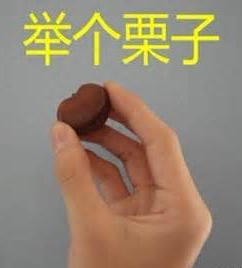
\includegraphics[width=0.6in]{jugelizi.png}\end{minipage}\begin{minipage}{0.76\textwidth}}
\def\eex{\end{minipage}}
\def\chtitle#1{\frametitle{\bch#1\ech}}
\def\bmat#1{\left(\begin{array}{#1}}
\def\emat{\end{array}\right)}
\def\bcase#1{\left\{\begin{array}{#1}}
\def\ecase{\end{array}\right.}
\def\bmini#1{\begin{minipage}{#1\textwidth}}
\def\emini{\end{minipage}}
\def\tbox#1{\begin{tcolorbox}#1\end{tcolorbox}}
\def\pfrac#1#2#3{\left(\frac{\partial #1}{\partial #2}\right)_{#3}}
%%symbols
\def\bropt{\,(\ \ \ )}
\def\sone{$\star$}
\def\stwo{$\star\star$}
\def\sthree{$\star\star\star$}
\def\sfour{$\star\star\star\star$}
\def\sfive{$\star\star\star\star\star$}
\def\rint{{\int_\leftrightarrow}}
\def\roint{{\oint_\leftrightarrow}}
\def\stdHf{{\textit{\r H}_f}}
\def\deltaH{{\Delta \textit{\r H}}}
\def\ii{{\dot{\imath}}}
\def\skipline{{\vskip0.1in}}
\def\skiplines{{\vskip0.2in}}
\def\lagr{{\mathcal{L}}}
\def\hamil{{\mathcal{H}}}
\def\vecv{{\mathbf{v}}}
\def\vecx{{\mathbf{x}}}
\def\vecy{{\mathbf{y}}}
\def\veck{{\mathbf{k}}}
\def\vecp{{\mathbf{p}}}
\def\vecn{{\mathbf{n}}}
\def\vecA{{\mathbf{A}}}
\def\vecP{{\mathbf{P}}}
\def\vecsigma{{\mathbf{\sigma}}}
\def\hatJn{{\hat{J_\vecn}}}
\def\hatJx{{\hat{J_x}}}
\def\hatJy{{\hat{J_y}}}
\def\hatJz{{\hat{J_z}}}
\def\hatj#1{\hat{J_{#1}}}
\def\hatphi{{\hat{\phi}}}
\def\hatq{{\hat{q}}}
\def\hatpi{{\hat{\pi}}}
\def\vel{\upsilon}
\def\Dint{{\mathcal{D}}}
\def\adag{{\hat{a}^\dagger}}
\def\bdag{{\hat{b}^\dagger}}
\def\cdag{{\hat{c}^\dagger}}
\def\ddag{{\hat{d}^\dagger}}
\def\hata{{\hat{a}}}
\def\hatb{{\hat{b}}}
\def\hatc{{\hat{c}}}
\def\hatd{{\hat{d}}}
\def\hatN{{\hat{N}}}
\def\hatH{{\hat{H}}}
\def\hatp{{\hat{p}}}
\def\Fup{{F^{\mu\nu}}}
\def\Fdown{{F_{\mu\nu}}}
\def\newl{\nonumber \\}
\def\vece{\mathrm{e}}
\def\calM{{\mathcal{M}}}
\def\calT{{\mathcal{T}}}
\def\calR{{\mathcal{R}}}
\def\barpsi{\bar{\psi}}
\def\baru{\bar{u}}
\def\barv{\bar{\upsilon}}
\def\qeq{\stackrel{?}{=}}
\def\torder#1{\mathcal{T}\left(#1\right)}
\def\rorder#1{\mathcal{R}\left(#1\right)}
\def\contr#1#2{\contraction{}{#1}{}{#2}#1#2}
\def\trof#1{\mathrm{Tr}\left(#1\right)}
\def\trace{\mathrm{Tr}}
\def\comm#1{\ \ \ \left(\mathrm{used}\ #1\right)}
\def\tcomm#1{\ \ \ (\text{#1})}
\def\slp{\slashed{p}}
\def\slk{\slashed{k}}
\def\calp{{\mathfrak{p}}}
\def\veccalp{\mathbf{\mathfrak{p}}}
\def\Tthree{T_{\tiny \textcircled{3}}}
\def\pthree{p_{\tiny \textcircled{3}}}
\def\dbar{{\,\mathchar'26\mkern-12mu d}}
\def\erf{\mathrm{erf}}
\def\const{\mathrm{constant}}
\def\pheat{\pfrac p{\ln T}V}
\def\vheat{\pfrac V{\ln T}p}
%%units
\def\fdeg{{^\circ \mathrm{F}}}
\def\cdeg{^\circ \mathrm{C}}
\def\atm{\,\mathrm{atm}}
\def\angstrom{\,\text{\AA}}
\def\SIL{\,\mathrm{L}}
\def\SIkm{\,\mathrm{km}}
\def\SIyr{\,\mathrm{yr}}
\def\SIGyr{\,\mathrm{Gyr}}
\def\SIV{\,\mathrm{V}}
\def\SImV{\,\mathrm{mV}}
\def\SIeV{\,\mathrm{eV}}
\def\SIkeV{\,\mathrm{keV}}
\def\SIMeV{\,\mathrm{MeV}}
\def\SIGeV{\,\mathrm{GeV}}
\def\SIcal{\,\mathrm{cal}}
\def\SIkcal{\,\mathrm{kcal}}
\def\SImol{\,\mathrm{mol}}
\def\SIN{\,\mathrm{N}}
\def\SIHz{\,\mathrm{Hz}}
\def\SIm{\,\mathrm{m}}
\def\SIcm{\,\mathrm{cm}}
\def\SIfm{\,\mathrm{fm}}
\def\SImm{\,\mathrm{mm}}
\def\SInm{\,\mathrm{nm}}
\def\SImum{\,\mathrm{\mu m}}
\def\SIJ{\,\mathrm{J}}
\def\SIW{\,\mathrm{W}}
\def\SIkJ{\,\mathrm{kJ}}
\def\SIs{\,\mathrm{s}}
\def\SIkg{\,\mathrm{kg}}
\def\SIg{\,\mathrm{g}}
\def\SIK{\,\mathrm{K}}
\def\SImmHg{\,\mathrm{mmHg}}
\def\SIPa{\,\mathrm{Pa}}
\def\secpage#1#2{\begin{frame}\bch\bcenter{\bf \Huge #1} \skipline \tbox{\bcenter #2\ecenter}\ecenter\ech\end{frame}}

\graphicspath{{figures/}}


\newcommand{\field}{\mathscr{F}}

\newcommand{\reals}{\mathbb{R}}
\newcommand{\complexs}{\mathbb{C}}
\newcommand{\ints}{\mathbb{Z}}
%\newcommand{\dim}{\mathrm{dim\ }}
\newcommand{\diag}{\mathrm{diag \ }}
\newcommand{\up}{\uparrow}
\newcommand{\down}{\downarrow}
\newcommand{\su}{\mathfrak{su}}
\newcommand{\so}{\mathfrak{so}}
\newcommand{\tr}{\mathrm{tr\ }}
\newcommand{\card}{\mathrm{card \ }}

\newtheorem{thm}{定理}[section]
\newtheorem{axm}{公理}[section]
\newtheorem{dfn}{定义}[section]
\newtheorem{experience}{经验}[section]


%\cpic{<尺寸>}{<文件名>}}用于生成居中的图片。
\newcommand{\cpic}[2]{
\begin{center}
\includegraphics[scale=#1]{#2}
\end{center}
}

%\cpicn{<尺寸>}{<文件名>}{<注释>}用于生成居中且带有注释的图片,其label为图片名。
\newcommand{\cpicn}[3]
{
\begin{figure}[h!]
\cpic{#1}{#2}
\caption{#3\label{#2}}
\end{figure}
}

\title{Group Theory\\ The Poor Man Finds His Roots}
  \author{Haoting Xu}
  \date{\today}


\begin{document}

\begin{frame}
 
\maketitle

%\vskip 0.2in
\begin{center}
xuht9@mail2.sysu.edu.cn
\vskip 0.1in
{\tiny \url{https://github.com/HaotingXu/seminar_lec} }\\
\end{center}
\end{frame}
\section{Introduction and Review}
\secpage{Introduction and Review}{吹水和复习}

\begin{frame}\frametitle{Introduction}
这一章我们来学习如何处理一般的李代数。在那之前我们需要看一些具体的例子找找感觉。这一讲全在算具体的例子找感觉,所以特别水。
\end{frame}
\begin{frame}\frametitle{回到$SU(2)$}
$SU(2)$的生成元是三个泡利矩阵$\frac12\sigma_i$,对角化$\sigma_3 = \begin{pmatrix} 1&0 \\ 0& -1\end{pmatrix}$,定义上升矩阵
\be
\frac12 \sigma_{1+i2} = 
\begin{pmatrix}
0&1 \\
0 &0 
\end{pmatrix}
\ee
于是从对易关系$[\frac12 \sigma_3,\frac12 \sigma_{1+i2}]=\frac12 \sigma_{1+i2}$,我们可以得知一维的根向量。
\end{frame}

\begin{frame}\frametitle{$\su(3)$的根向量}
  回忆$\su(3)$生成元是无迹厄米矩阵的集合,经过一定的线性组合之后得到八个盖尔曼矩阵,他们按$\mathrm{tr}\lambda_a\lambda_b = 2\delta_{ab}$归一化。
  \be
  \lambda_1 =
  \begin{pmatrix} 0&1&0 \\ 1&0&0 \\ 0&0&0\\
  \end{pmatrix}
  ,\, \lambda_2 =
  \begin{pmatrix} 0&-i&0 \\ i&0&0 \\ 0&0&0\\
  \end{pmatrix}
  \lambda_4 =
  \begin{pmatrix} 0&0&1 \\ 0&0&0 \\ 1&0&0\\
  \end{pmatrix}
  ,\, \lambda_5 =
  \begin{pmatrix} 0&0&-i \\ 0&0&0 \\ i&0&0\\
  \end{pmatrix}
  \ee
  \be
  \lambda_6 =
  \begin{pmatrix} 0&0&0 \\ 0&0&1 \\ 0&1&0\\
  \end{pmatrix}
  ,\, \lambda_7 =
  \begin{pmatrix} 0&0&0 \\ 0&0&-i \\ 0&i&0\\
  \end{pmatrix}
  \lambda_3 =
  \begin{pmatrix} 1&0&0 \\ 0&-1&0 \\ 0&0&0\\
  \end{pmatrix}
  ,\, \lambda_8 =\frac{1}{\sqrt{3}}
  \begin{pmatrix} 1&0&0 \\ 0&1&0 \\ 0&0&-2\\
  \end{pmatrix}
  \ee
\end{frame}
\begin{frame}\frametitle{盖尔曼矩阵}
  仔细观察盖尔曼矩阵,我们发现
  \begin{itemize}
  \item $\lambda_1,\lambda_2$是所谓$1-2$泡利矩阵
  \item $\lambda_4,\lambda_5$是所谓$1-3$泡利矩阵。
  \item $\lambda_6,\lambda_7$是所谓$2-3$泡利矩阵。
  \item $\lambda_3,\lambda_8$是两个对角矩阵,任何无迹厄米对角矩阵都可以写成$\lambda_3,\lambda_8$的线性组合。一个代数中可同时对角化的生成元数目被成为代数的rank,用$l$表示。
  \end{itemize}
  因此$SU(3)$有两个可以对角化的生成元,我们说$SU(3)$的秩是$2$。引入记号$\frac{1}{2}\lambda_{1+i2},\frac{1}{2}\lambda_{4+i5},\frac12\lambda_{6+i7}$,通过计算与$\frac12\lambda_3$和$\frac12\lambda_8$的对易关系,我们便可以得到根向量。  
\end{frame}
\begin{frame}\frametitle{得到$SU(3)$的根向量}
因为这些生成元其实都是$x,y$泡利矩阵,所以在计算根向量的时候我们不必要每次计算$3\times 3$的乘法。而只用计算$2\times 2$矩阵的乘法就可以了。
\begin{itemize}
  \item 例如,$\frac{1}{2}\lambda_{1+i2} = \begin{pmatrix} 0&1&0 \\ 0&0&0 \\ 0&0&0\\
  \end{pmatrix}$
  它是由$1-2$泡利矩阵得到的生成元,只有左上角那一块不是$0$,因此当计算与$\frac{1}{2}\lambda_8$的对易关系时只需要使用左上角的$2\times2$方块进行计算。
  \item 又如,$\frac{1}{2}\lambda_{4+i5} = \begin{pmatrix} 0&0&1 \\ 0&0&0 \\ 0&0&0\\
  \end{pmatrix}$,我们只需要提取出$1-3$方块进行计算,这时对应计算的$\lambda_3,\lambda_8$分别为$\begin{pmatrix} 1&0\\0&0\end{pmatrix},\,\begin{pmatrix} 1&0\\0&-2\end{pmatrix}$
  \end{itemize}
\end{frame}
\begin{frame}\frametitle{Determining roots}
上面的思考启发我们来算一个一般的公式
\be
\left[\begin{pmatrix} 1&0\\0&-n\end{pmatrix},\begin{pmatrix} 0&1\\0&0\end{pmatrix}\right] =\left[\begin{pmatrix} n+1&0\\0&0\end{pmatrix},\begin{pmatrix} 0&1\\0&0\end{pmatrix}\right]=(n+1)\begin{pmatrix}0&1\\0&0\end{pmatrix}
\ee
对于$\frac12\lambda_{4+i5}$与$\lambda_3$的对易关系,我们取$n=0$,对于它和$\lambda_8$的对易关系,我们取$n+2$。事实上,如果我们记住一些归一化常数,我们瞬间就可以写出$\frac12\lambda_{4+i5}$对应的根向量
\be
\frac{1}{2}\left((0+1),\frac{1}{\sqrt{3}}(2+1)\right)=\frac{1}{2}(1,\sqrt{3})
\ee
进一步我们发现$\frac12 \lambda_{6+i7}$对应的根向量是$\frac12(-1,\sqrt{3})$,最终我们得到了三个根向量$(1,0),\frac{1}{2}(1,\sqrt{3}),\frac12(-1,\sqrt{3})$。它们的模长都是1,而且他们内积的绝对值都是$\frac12$,即两两之间夹角为$60^{\circ}$或$120^{\circ}$。
\end{frame}

\begin{frame}\frametitle{Presses onward to $SU(4)$ easily}
通过上面的例子,我们知道了下面的经验
\begin{experience}
计算对易关系,只需要计算$2\times 2$矩阵就行了。
\end{experience}
现在我们考虑$SU(4)$的情况,我们知道$SU(N)$群的生成元是无迹厄米矩阵,因此我们掐指一算,$SU(4)$群有$2\times(3+2+1)+3=15$个生成元,如果按照之前的形式,我们有三个对角化的矩阵
\be
\lambda_3 = 
\begin{pmatrix}
1&&& \\
&-1&& \\
&&&&\\
&&&&
\end{pmatrix}
,\,\lambda_8 = 
\begin{pmatrix}
1&&&\\
&1&&\\
&&-2&\\
&&&&
\end{pmatrix}
,\,\lambda_{15}=
\begin{pmatrix}
1&&&\\
&1&&\\
&&1&\\
&&&-3
\end{pmatrix}
\ee
\end{frame}
\begin{frame}\frametitle{$SU(4)$根向量}
三个对角化的矩阵意味着它的参数空间是三维的。之前的升降算符,例如$\begin{pmatrix} &&&\\&&1&\\&&&\\&&&\end{pmatrix}$都在原来的参数空间里面,新多出来的就是4分量的东西,例如$\begin{pmatrix} &&&1\\&&&\\&&&\\&&&\end{pmatrix}$,请试着计算它对应的根向量。
\end{frame}
\begin{frame}\frametitle{$SU(N)$}
计算结果为那个矩阵对应的根向量为$\frac12(1,\frac{1}{\sqrt{3}},2\sqrt{\frac{2}{3}})$,可以证明,它的模长是1,它与其他根向量的夹角是$60^\circ$或者$120^\circ$。
\begin{problem}[$SU(5)$群的根图]
For fun, you could work out $SU(5)$ and see whether the pattern persists.
\end{problem}
注:我们这本书的最终章将学习,$SU(5)$是大统一理论(grand unified theory)的对称群。
\end{frame}
\section{Roots and Weights for Orthogonal Unitary and Symplectic Algebras}
\secpage{Roots and Weights for Orthogonal, Unitary and Symplectic Algebras}{$H^1 = \diag(1,-1,0,0,\cdots,0,0)$}
\begin{frame}\frametitle{概念复习}
  \begin{dfn}[Positive Roots]
    一个根是正的,如果它对应向量的第一个非零实数分量为正。
  \end{dfn}
  说一个根是不是正的,与它本征值选取顺序有关,我们取了$(i_3,i_8)$,但原则上,也可以反着取。如果像原来那样取,则正根为$\vec{V}_+,\,\vec{I}_+,\,\vec{U}_-$,且有$\vec{I}_+ = \vec{V}_+ + \vec{U}_-$,我们有下面的定义
  \begin{dfn}[Simple roots]
    给定一个$l$维空间正根的集合,一个子集被称作简单的,如果子集中的任何正根都可以写成简单根的非负系数线性组合。
  \end{dfn}
\end{frame}
\begin{frame}\frametitle{获得基础表示根向量的一般方法}
一般来说采取如下步骤
\begin{enumerate}[(1)]
  \item 找到可同时对角化的生成元,记作$H^i$,使用$\tr(H^iH^j)=\delta^{ij}$归一化。
  \item 直接从$H^i$中读出weights。
  \item 从weight diagram中读出根。
  \item 选定一种方向的顺序,从根中读出正根。
  \item 从正根中选出简单根。
\end{enumerate}
\end{frame}
\begin{frame}\frametitle{一个简单的例子——$SU(3)$}
$SU(3)$群的两个可同时对角化的矩阵为
\be
H^1 = \diag(1,-1,0)/\sqrt{2}
\ee
\be
H^2 = \diag(1,1,-2)/\sqrt{6}
\ee
注意这里按照$\tr(H^iH^j)=\delta^{ij}$归一化。于是$SU(3)$的weights生活在二维空间中,从上面的生成元可直接读出weights的坐标分量分别为
\bea
w^1 &=& \frac{1}{\sqrt{2}}(1,\frac{1}{\sqrt{3}})\\
w^2 &=& \frac{1}{\sqrt{2}}(-1,\frac{1}{\sqrt{3}})\\
w^3 &=& \frac{1}{\sqrt{2}}(0,-\frac{2}{\sqrt{3}})
\eea
其中$w_1,w_2,w_3$分别对应于上夸克、下夸克和奇异夸克。可以看到,他们形成等边三角形。
\end{frame}
\begin{frame}\frametitle{正根和简单根}
接下来我们求根
\bea
\alpha^1&\equiv& w^1 - w^2 = \sqrt{2}(1,0)\\
 \alpha^2&\equiv& w^2 - w^3 = \frac{1}{\sqrt{2}}(-1,\sqrt{3})\\
  \alpha^3&\equiv& w^1 - w^3 = \frac{1}{\sqrt{2}}(1,\sqrt{3}).
\eea
数学家这样选他们的方向来判断正根,他们选取$H_2$在前,$H_1$在后,这样正根就可以写成
\be
w^m-w^n\,\,\mathrm{for\,\,all\,\,  } m<n
\ee
简单根似乎很难写成这样的形式,不过不久之后我们将会看到一种更加舒适的写法。
\end{frame}
\begin{frame}\frametitle{向$SO(N)$出发}
现在我们有足够的储备来研究$SO(N)$群了,我们一会就会发现,奇数的情况和偶数的情况要单独讨论。
\end{frame}
\begin{frame}\frametitle{第二个例子$SO(4)$}
我们来研究$SO(4)$的根图。首先,我们回忆$SO(N)$群的生成元是$J = -i\mathcal{J}$,其中$\mathcal{J}$是一个反对称矩阵。对于$SO(4)$群,可同时对角化的两个生成元的一种选择是
\bea
H^1 &=& \diag(1,-1,0,0)\\
H^2 &=& \diag(0,0,1,-1)
\eea
这是因为他们分别旋转$1-2$平面和$3-4$平面,没有第三个生成元和他们同时对易。
这相当于对$(x_1\pm i x_2,x_3\pm ix_4)$进行操作。然后我们读出weights
\be
w^1 = (1,0),\,\,\, w^2 = (-1,0),\,\,\,w^3 = (0,1),\,\,\,w^4=(0,-1)
\ee
\end{frame}
\begin{frame}\frametitle{正方形出现了!}
进而求出根向量
\bea
\alpha^1&\equiv& w^1 - w^4 = (1,1),\,\,
\alpha^2\equiv w^1 - w^3 = (1,-1)\\
\alpha^3&\equiv& w^4 - w^1 = (-1,-1),\,\,
\alpha^4\equiv w^3 - w^1 = (-1,1)
\eea
把weights和根向量画出来,我们的老朋友,正方形出现了。
\cpicn{0.25}{SO4}{$\so (4)$代数的根图}
\end{frame}
\begin{frame}\frametitle{思考题}
\cpic{0.3}{think2}
在$SU(3)$群中,我们的根向量可以沟通所有的weights,但是你有没有发现在$SO(4)$群中却没有沟通$w^1,w^2$的roots,这是为什么呢?难道我们把它漏掉了?
\end{frame}
\begin{frame}\frametitle{思考题解答}
\cpic{0.3}{think}
前面说过,如果同时对角化$H^1,H^2$,相当于对$(x_1\pm ix_2,x_3\pm ix_4)$进行旋转,而这种旋转是没法沟通第一个坐标和第二个坐标。
\end{frame}
\begin{frame}\frametitle{45度的偏差}
我们发现$w$的方向和$\alpha$的方向不太一致,而是偏差了45度,这意味着
\be
SO(4)\simeq SU(2)\otimes SU(2)
\ee
这个在第四章讲过(或是在相对论量子力学的第一章)。
\end{frame}
\begin{frame}\frametitle{$\so(4)$的正根和简单根}
我们可以把$\alpha$写成一个简单的形式,如果用$e^i$来表示$l$维空间上的基底,则$\alpha$可以表示成
\be
\pm e^1\pm e^2 \text{(signs uncorrelated)}
\ee
很容易发现,正根就是
\be
e^1\pm e^2
\ee
他们全是简单根。
\end{frame}
\begin{frame}\frametitle{$SO(5)$群}
我们再来看$SO(5)$群,我们仔细思考$SO(5)$的生成元,能同时对角化的矩阵也只有五个里面挑两个坐标,对角化之后是$\sigma_3$。但是挑选完成之后总会剩一个坐标。于是$SO(5)$的对角化的生成元和$SO(4)$几乎相同
\bea
H^1 &=& \diag(1,-1,0,0,0)\\
H^2 &=& \diag(0,0,1,-1,0)
\eea
因此$SO(5)$的根向量也生活在2维空间。我们可以瞬间得到weights,我们发现前四个weights和$SO(4)$是一样的,唯独多了一个
\be
w^5 = (0,0)
\ee
\end{frame}
\begin{frame}\frametitle{短根和长根}
将weight diagram和根图画出来是这个样子
\cpic{0.25}{SO5}
注意因为相同的原因,还是没有沟通$w^1,w^2$的根。但是这里我们看到了一个新的特性,那就是根的长度不一样。其中$\alpha^1,\alpha^2,\alpha^3,\alpha^4$的长度为$\sqrt{2}$,被称为长根(long roots)。而$\alpha^5,\alpha^6,\alpha^7,\alpha^8$的长度为1,被成为短根(short roots)。

注意如果采取不同的对$H$的归一化关系,根的具体长度将变得不同,但是具体长根和短根长度的比值是不变的——它不依赖于归一化的选取。
\end{frame}
\begin{frame}\frametitle{正根和简单根}
八个根向量可以写成
\be
\pm e^1 \pm e^2 \text{ (signs uncorrelated)},\pm e^1,\,\pm e^2
\ee
显然,正根为
\be
e^1\pm e^2,\,e^1,\,e^2
\ee
简单根为
\be
e^1-e^2,e^2
\ee
\end{frame}
\begin{frame}\frametitle{思考题}
\cpic{0.3}{think3}
尝试写出$SO(6)$的weights, roots, positive roots and simple roots.

从上面的例子我们能体会到,奇数的情况和偶数的情况是不同的。
\end{frame}
\begin{frame}\frametitle{$SO(2l)$}
现在,我们来处理$SO(2l)$的情况,可同时对角化的生成元为
\bea
H^1 &=& \diag(1,-1,0,0,\cdots,0,0)\\
H^2 &=& \diag(0,0,1,-1,\cdots,0,0)\\
&\vdots & \\
H^l &=& \diag(0,0,0,0,\cdots,1,-1)
\eea
可以读出它的$2l$个weights
\be
w^1=\begin{pmatrix}1\\0\\ \vdots \\ 0 \end{pmatrix},\,
w^2=\begin{pmatrix}-1\\0\\ \vdots \\ 0 \end{pmatrix},\,
w^{2l-1} = \begin{pmatrix} 0\\0\\ \vdots \\ 1\end{pmatrix},\,
w^{2l} = \begin{pmatrix} 0\\0\\ \vdots \\ -1\end{pmatrix}
\ee
他们生活在$l$维空间当中,他们可以记作$\pm e^i,\text{ for }i=1,\cdots,l$.
\end{frame}
\begin{frame}\frametitle{根}
于是根可以表述为$\pm e^i \pm e^j\text{( signs uncorrelated )},\, (i<j)$,我们来数一数根的数目为$4\times \sum_{m=1}^l m-1 = 2l(l-1)$,总共的生成元数目
\be
2l(l-1)+l=2l(2l-1)/2
\ee
取正根为$e^i\pm e^j$,则简单根为
\be
e^{i-1}-e^i,\, e^{l-1}+e^l,\,\, (i=2,\cdots,l)
\ee
\end{frame}
\begin{frame}\frametitle{简单根的证明}
我们来证明所有的正根$e^m\pm e^n,\,(m<n)$都可以写成所有简单根的非负线性组合。首先有
\be
e^m-e^n = (e^m-e^{m+1})+(e^{m+1}-e^{m+2})+\cdots+(e^{n-1}-e^n)
\ee
对于加法,我们将最后一项改造一下
\be
e^m+e^n = (e^m-e^{m+1})+(e^{m+1}-e^{m+2})+\cdots+(e^{n-1}-e^n)+(e^n-e^l)+(e^n+e^l)
\ee
再利用
\bea
e^n-e^l &=& (e^n-e^{n+1})+(e^{n+1}-e^{n+2})+\cdots+(e^{l-1}-e^l)\\
e^n+e^l &=& (e^n-e^{n+1})+(e^{n+1}-e^{n+2})+\cdots+(e^{l-1}+e^{l})
\eea
这样所有的正根就全写成简单根的线性组合了。
\end{frame}
\begin{frame}\frametitle{$SO(2l+1)$}
对于$SO(2l+1)$重复同样的操作。得到多了一个根$w^{2l+1}=(0,0,\cdots,0)$,根可以表示为
\be
\pm e^i \pm e^j\text{( signs uncorrelated )},\, (i<j),\,\pm e^i
\ee

下一步,检查生成元个数为$2l(2l+1)/2$。最后,得到正根为
$e^i\pm e^j,\,e^i$
,简单根为
\be
e^{i-1}-e^i,\, e^l
\ee
尝试证明简单根是简单根。
\cpic{0.5}{nimashinima}
\end{frame}
\begin{frame}\frametitle{$SU(N)$群的根}
$SU(N)$群可同时对角化的生成元为
\bea
H^1 &=&\diag(1,-1,0,\cdots,0)/\sqrt{2}\\
H^2 &=& \diag(1,1,-2,\cdots,0)/\sqrt{6}\\
&\vdots & \\
H^i &=& \diag(\underbrace{1,1,\cdots,1}_{i},-i,0,\cdots,0)/\sqrt{i(i+1)}\\
H^l &=& \diag(0,0,0,0,\cdots,1,-1)/\sqrt{l(l+1)}
\eea
$SU(N)$的根向量生活在$l=N-1$维空间。可以读出$w^j$的第$i$个分量是$\left(H^i\right)_{jj}$。
\end{frame}
\begin{frame}\frametitle{根向量}
$SU(N)$群的根向量为$w^m-w^n$,其中$m,n=1,\cdots,N$。正根可以表示为
$w^m-w^n$,其中$m<n$。简单根有$N-1$个,为
\be
w^m - w^{m+1} \text{ for }m=1,2,\cdots,N-1
\ee
\end{frame}
\begin{frame}\frametitle{从线段到等边三角形到正四面体}
\cpic{0.3}{think2}
试着推导出$SU(4)$的根图,并发现它是一个正四面体。试着写出$SU(4)$的三个简单根,定义为
\bea
\alpha^1 &\equiv& w^1-w^2\\
\alpha^2 &\equiv& w^2-w^3\\
\alpha^3 &\equiv& w^3-w^4
\eea
并证明$\left(\alpha^1\right)^2=\left(\alpha^2\right)^2=\left(\alpha^3\right)^2=2$且$\alpha^1\cdot \alpha^2 = -1,\,\,\alpha^2\cdot \alpha^3 = -1$。$\alpha^1\cdot \alpha^3=0$,因为正四面体的两条边是垂直的。
\end{frame}
\begin{frame}\frametitle{另一个优美的表示方法}
我们发现到目前为止,$SU(N)$群的根向量都满足
\be
\left(\alpha^i\right)^2=2,\,\, \alpha^{i}\cdot \alpha^{i+1}=-1
\ee
其中$i=1,\cdots,l-1$。考虑$(l+1)$维空间中的基底$e^i$,我们发现
\be
(e^i - e^{i+1})^2=1+1=2,\,\, (e^i-e^{i+1})\cdot (e^j - e^{j+1})=\left\{
\begin{aligned}
-1&,&\,j=i\pm 1\\
0&,&\, \text{otherwise}
\end{aligned}
\right.
\ee
所以$l$个$SU(l+1)$的简单根为
\be
\alpha^i\equiv e^i - e^{i+1},\, i=1,\cdots , l
\ee
\end{frame}
\begin{frame}\frametitle{辛群复习}
辛群就是在辛流形上保内积不变的变换的集合。辛群满足$R^TJR=J$。幺正辛群的生成元为
\be
H = \begin{pmatrix} iA+S_3 & S_1-iS_2 \\ S_1+iS_2 & iA-S_3 \end{pmatrix}= iA\otimes I +iS_i\otimes \sigma_i
\ee
小朋友快来猜一猜,上面哪个是已经同时对角化了的生成元?
\cpic{0.3}{why}
\end{frame}
\begin{frame}\frametitle{}
对角化的生成元为
\be
H^i = u^i\otimes \sigma_3 = \begin{pmatrix} u^i & 0 \\ 0 &-u^i \end{pmatrix}
\ee
\cpic{0.3}{think4}
对于$Sp(4)$的情况,得到根图。注意这与$SO(2l)$的情况不同,可以有沟通$w^1,w^3$的根。
\end{frame}
\begin{frame}\frametitle{Positive roots and Simple roots}
得到的根图如图
\cpicn{0.3}{Sp4}{$Sp(4)$的根图}
注意到如果将此图旋转$45^\circ$,就会得到$SO(5)$的根图,这暗示了
\be
Sp(4)\simeq SO(5)
\ee
\end{frame}
\begin{frame}\frametitle{Positive roots and Simple roots}
对于$Sp(2l)$群,我们得到它的根为
\be
\pm e^i \pm e^j,\,\, \pm 2e^i ,\,\, i,j=1,\cdots,l
\ee
positive roots
\be
e^i\pm e^j,\,\, 2e^i
\ee
simple roots
\be
e^{i-1}-e^i ,\,\, i=2,\cdots,l \text{ and } 2e^l
\ee
最后,证实$Sp(2l)$有$l^2$个正根,$l(2l+1)$个生成元。
\end{frame}
\section{summary}
\begin{frame}\frametitle{总结}
最后,我们将这节课学的根都列在下面的表中。
\begin{table}
  \begin{center}
  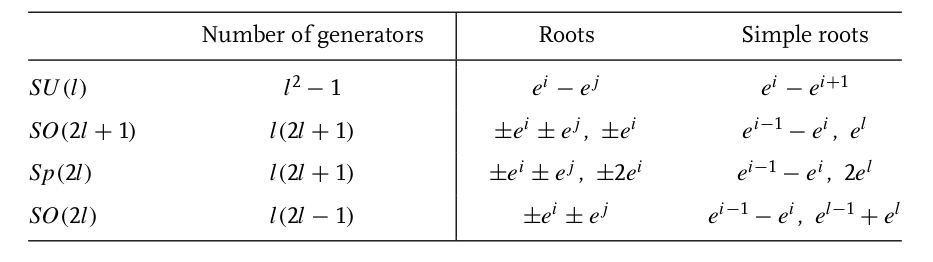
\includegraphics[scale=0.3]{table}
  \end{center}
  \caption{The four families we have studied.}
\end{table}

\end{frame}
\end{document}
